\documentclass{article}

% ==========================================================
%  Pacchetti importati
% ==========================================================
\usepackage[italian]{babel}
\usepackage[letterpaper,top=2cm,bottom=2cm,left=3cm,right=3cm,marginparwidth=1.75cm]{geometry}
\usepackage{amsmath}
\usepackage{graphicx}
\usepackage{subcaption}
\usepackage{textcomp}
\usepackage{float}
\usepackage{ragged2e}
\usepackage[export]{adjustbox}
\usepackage[table, dvipsnames]{xcolor}
\usepackage{tcolorbox}
\usepackage{tabularx}
\usepackage{fancyhdr}
\usepackage{lastpage}
\usepackage[labelfont=bf, font=small]{caption}
\usepackage{pifont}

% ==========================================================
% Informazioni pdf
% ==========================================================
\usepackage[colorlinks=true, allcolors=blue,
            pdfauthor={Matteo Drago},
            pdftitle={Malga Valletta Alta},
            pdfsubject={Diario bivacchi e trekking},
            pdfkeywords={bivacco, montagna, trekking, diario},
            pdfproducer={LaTeX},
            pdfcreator={TeX Live 2025},
            pdflang={it-IT},
            pdfdisplaydoctitle=true,
            pdfstartview=FitH,
            pdfpagemode=UseOutlines]{hyperref}
            
\title{\textbf{Malga Valletta Alta - 1887 m s.l.m}}
\author{Matteo Drago}

% ==========================================================
%  Impostazioni per header e footer in ogni pagina
% ==========================================================
\pagestyle{fancy}
\fancyhf{} % Pulisce tutti i campi di intestazione e piè di pagina
\fancyhead[R]{
\includegraphics[height=1.5cm]{images/toothless.jpeg}} % Posiziona il logo a destra (R) nell'intestazione
\fancyfoot[C]{\small\itshape Malga Valletta Alta — Dicembre 2022}
\fancyfoot[R]{Pagina \thepage\ di \pageref{LastPage}} % lato destro
\renewcommand{\headrulewidth}{0pt} % Rimuove la linea orizzontale nell'intestazione (opzionale)

%==========================================================

\begin{document}
\maketitle
\thispagestyle{fancy}


% ==========================================================
%  Abstract
% ==========================================================
\begin{abstract}
Questo documento raccoglie e organizza le informazioni che ho acquisito nel corso degli anni sui bivacchi, basate sulle mie esperienze dirette. Sebbene non si proponga come una guida esaustiva e perfetta, offre il minimo indispensabile per una buona vita in bivacco, con consigli pratici e diretti per chiunque desideri affrontare al meglio queste pazze ma piacevoli avventure.
\end{abstract}

\section{Il bivacco}

% ==========================================================
% Immagine a sinistra, testo a destra allineato in alto
% ==========================================================
\noindent
\begin{minipage}[t]{0.45\textwidth}
  \vspace{0pt} % forza l'allineamento in alto
  
\includegraphics[width=\linewidth, frame]{images/bivacco.jpg}
\end{minipage}
\hfill
\begin{minipage}[t]{0.5\textwidth}
  \vspace{0pt} % forza l'allineamento in alto
  
  
  Regione\\
  \textbf{\large Trentino-Alto Adige}
  \\[1em] % Aggiunge una riga vuota qui
  Provincia/Comune\\
  \textbf{\large Trento / Valfloriana}
  \\[1em] % Aggiunge una riga vuota qui
  Gruppo montuoso\\
  \textbf{\large Catena del Lagorai}
  \\[1em] % Aggiunge una riga vuota qui
  Quota\\  
  \textbf{\large 1887 m s.l.m.}
  \\[1em] % Aggiunge una riga vuota qui
  Coordinate\\  
  \textbf{\large \href{https://maps.google.com/?q=46.18633,11.39534}{46.18633° N, 11.39534° E}}
  \\[1em] % Aggiunge una riga vuota qui
  Apertura\\  
  \textbf{\large Non gestito, sempre aperto}

\end{minipage}

\subsection{Caratteristiche}
La malga Valletta Alta è un rifugio alpino con caratteristiche di bivacco attrezzato e assieme alla malga Fornasa alta, la cugina praticamente, rappresentano quello che molti definiscono un gioiello di struttura.

Il bivacco è suddiviso in 2 piani:
\begin{itemize}
    \item \textbf{Piano terra}: una stanza con tavolo e panche, una dispensa fornita, una cucina a gas e una stufa.
    \item \textbf{Piano superiore}: un soppalco con circa una decina di posti disponibili (non ricordo la presenza di materassi o brande).
    \item \textbf{Spazio esterno}: con fonte d'acqua attiva sia in estate che in inverno, una legnaia fornita sul lato del bivacco e sulla strada per arrivare si presenta anche un "bagno-latrina".
\end{itemize}

La stufa presente è in grado di riscaldare molto facilmente tutto il bivacco e ricavare la legna non è complesso grazie alla presenza del bosco.

\section{Come ci siamo arrivati}
Il bivacco è stato inserito in un giro di tre giorni che comprendeva la malga Valletta Alta e la malga Fornasa Alta.

Abbiamo parcheggiato l’auto sulla strada Provinciale 31 del Manghen, (non ho un punto specifico data la presenza di molta neve sulla strada, siamo saliti fino a quando ci era permesso, comunque potete vedere la traccia gpx) e da lì ci siamo incamminati fino a raggiungere la \href{https://maps.google.com/?q=46.18633,11.39534}{malga Valletta Alta}. Il giorno successivo siamo ripartiti in direzione della \href{https://maps.google.com/?q=46.17745,11.40920}{malga Fornasa Alta} per poi terminare il giro il terzo giorno, tornando al parcheggio.
Lascio le informazioni del giro completo dei 3 giorni.

\begin{figure}[htbp!]
    \centering
    % Colonna di sinistra, allineata in alto
    \begin{subfigure}[t]{0.45\textwidth}
        \centering
        \vspace{0pt} % Forziamo l'allineamento in alto
        
\includegraphics[width=\textwidth]{images/sentiero_mapsMe.jpg}
        \caption{Sentiero su Maps.Me.}
        \vspace{1em}
        \textbf{Percorso:}\\
        Giorno 1: 8,56 km $\Longleftrightarrow$, 730 m $\uparrow$, 0 m $\Downarrow$
        Giorno 2: 4,14 km $\Longleftrightarrow$, 420 m $\uparrow$, 350 m $\Downarrow$
        Giorno 3: 10,3 km $\Longleftrightarrow$, 110 m $\uparrow$, 910 m $\Downarrow$
    \end{subfigure}
    \hfill
    % Colonna di destra, allineata in alto
    \begin{subfigure}[t]{0.45\textwidth}
        \centering
        \vspace{0pt} % Forziamo l'allineamento in alto anche qui
        
\includegraphics[width=\textwidth]{images/sentiero_komoot.png}
        \caption{Sentiero su Komoot.}
        \vspace{4em} % Aggiunge un po' di spazio tra le due foto
        
\includegraphics[width=\textwidth]{images/profilo_altimetrico.jpg}
        \caption{Profilo altimetrico del percorso.}
        \end{subfigure}
    % Didascalia generale per l'intera figura
    \caption{Il sentiero e i dettagli del percorso.}
\end{figure}


% ==========================================================
%  Non ti scordar di me
% ==========================================================
\section{Non ti scordar di me}
\begin{tcolorbox}[colback=yellow!15!white, colframe=yellow!80!black]
\textbf{\textcolor{BurntOrange}{Ricorda: il bivacco è un bene comune. Il suo futuro dipende dal rispetto e dal senso civico dei visitatori. Usalo con cura e lascialo più pulito di come l'hai trovato.}}    
\end{tcolorbox}



\section{Esperienza personale}
La complessità di questo giro si è rivelata \textbf{molto elevata}.
Siamo partiti con poche ciaspole rispetto a quelle disponibili, convinti che la neve non fosse molta e che, in ogni caso, fosse piuttosto compatta. Mai scelta fu più sbagliata: lungo il tratto stradale la neve era effettivamente dura e battuta, ma appena ci siamo addentrati nei sentieri è diventata più abbondante e soffice.
Camminare con le ciaspole non è stato semplice, e persino restare in equilibrio da fermi richiedeva uno sforzo notevole. 

Il \textbf{primo giorno} è stato comunque gestibile: l’unica vera difficoltà è stata la salita finale verso il bivacco, che per fortuna abbiamo trovato libero e accogliente, permettendoci di riposare in vista della tappa successiva verso la malga Fornasa Alta.

Il \textbf{secondo giorno} si è rivelato molto più impegnativo. La salita era ripidissima: chi non aveva le ciaspole letteralmente “nuotava nella neve”. Abbiamo raggiunto la vetta con molta fatica e poi il bivacco, ma solo verso le 17:00, partendo alle 10:00 e senza riuscire a fermarci per pranzo per mancanza di un luogo adatto alla sosta.

Il \textbf{terzo giorno} ci ha messo di fronte a un’ulteriore difficoltà. Il sentiero che avremmo dovuto seguire era completamente ostruito dagli alberi abbattuti dalla tempesta Vaia: tronchi caduti e ramaglie bloccavano ogni passaggio. Abbiamo quindi dovuto improvvisare un percorso alternativo, districandoci tra rovi, salite ripide e deviazioni forzate. È stato un cammino lento e faticoso, ma alla fine siamo riusciti a ritornare al parcheggio, stanchi ma soddisfatti di aver concluso il giro.


\section{Alcune foto}

% Sezione Alcune foto

\begin{figure}[htbp!]
    \centering
    % Prima riga: Due foto (QUESTA È LA PRIMA FIGURA)
    \begin{subfigure}[b]{0.45\textwidth}
        
\includegraphics[width=\textwidth]{images/foto_sentiero.jpg}
        \caption{Sentiero.}
    \end{subfigure}
    \hfill
    \begin{subfigure}[b]{0.45\textwidth}
        
\includegraphics[width=\textwidth]{images/foto_paesaggio.jpg}
        \caption{Paesaggio.}
    \end{subfigure}
\end{figure}


\begin{figure}[H]
    \centering
    % Seconda riga: Tre foto (QUESTA È LA SECONDA FIGURA)
    \begin{subfigure}[b]{0.45\textwidth}
        
\includegraphics[width=\textwidth]{images/foto_paesaggio2.jpg}
        \caption{Altro paesaggio.}
    \end{subfigure}
    \hfill
    \begin{subfigure}[b]{0.45\textwidth}
        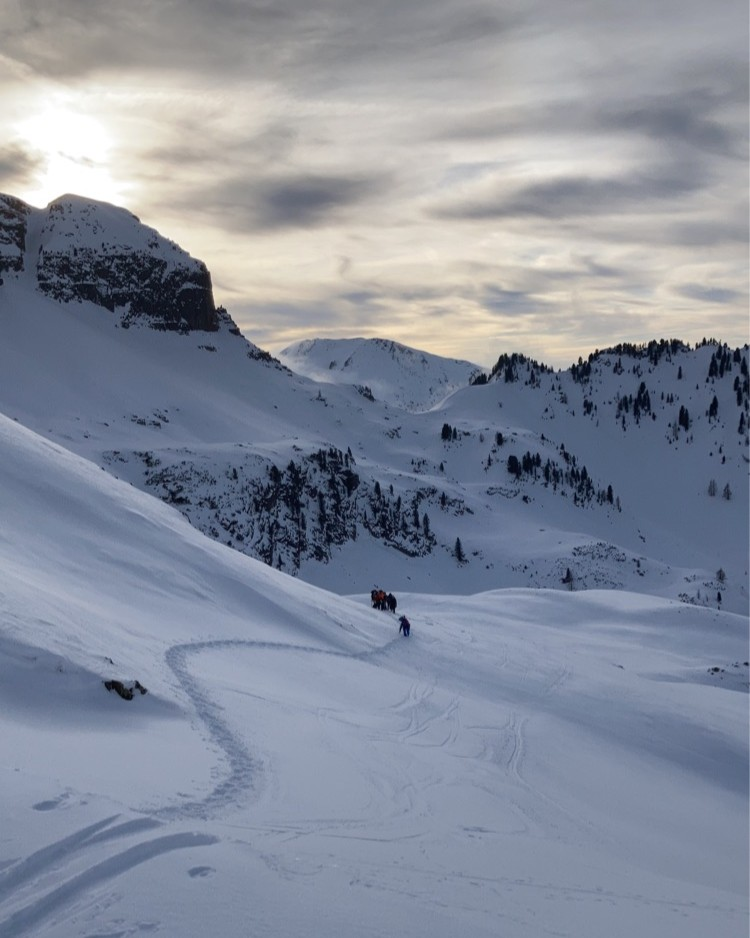
\includegraphics[width=\textwidth]{images/foto_sentiero2.JPG}
        \caption{Altro sentiero.}
    \end{subfigure}
    \hfill
\end{figure}

\begin{figure}[H]
    \centering
    % Seconda riga: Tre foto (QUESTA È LA SECONDA FIGURA)
    \begin{subfigure}[b]{0.45\textwidth}
        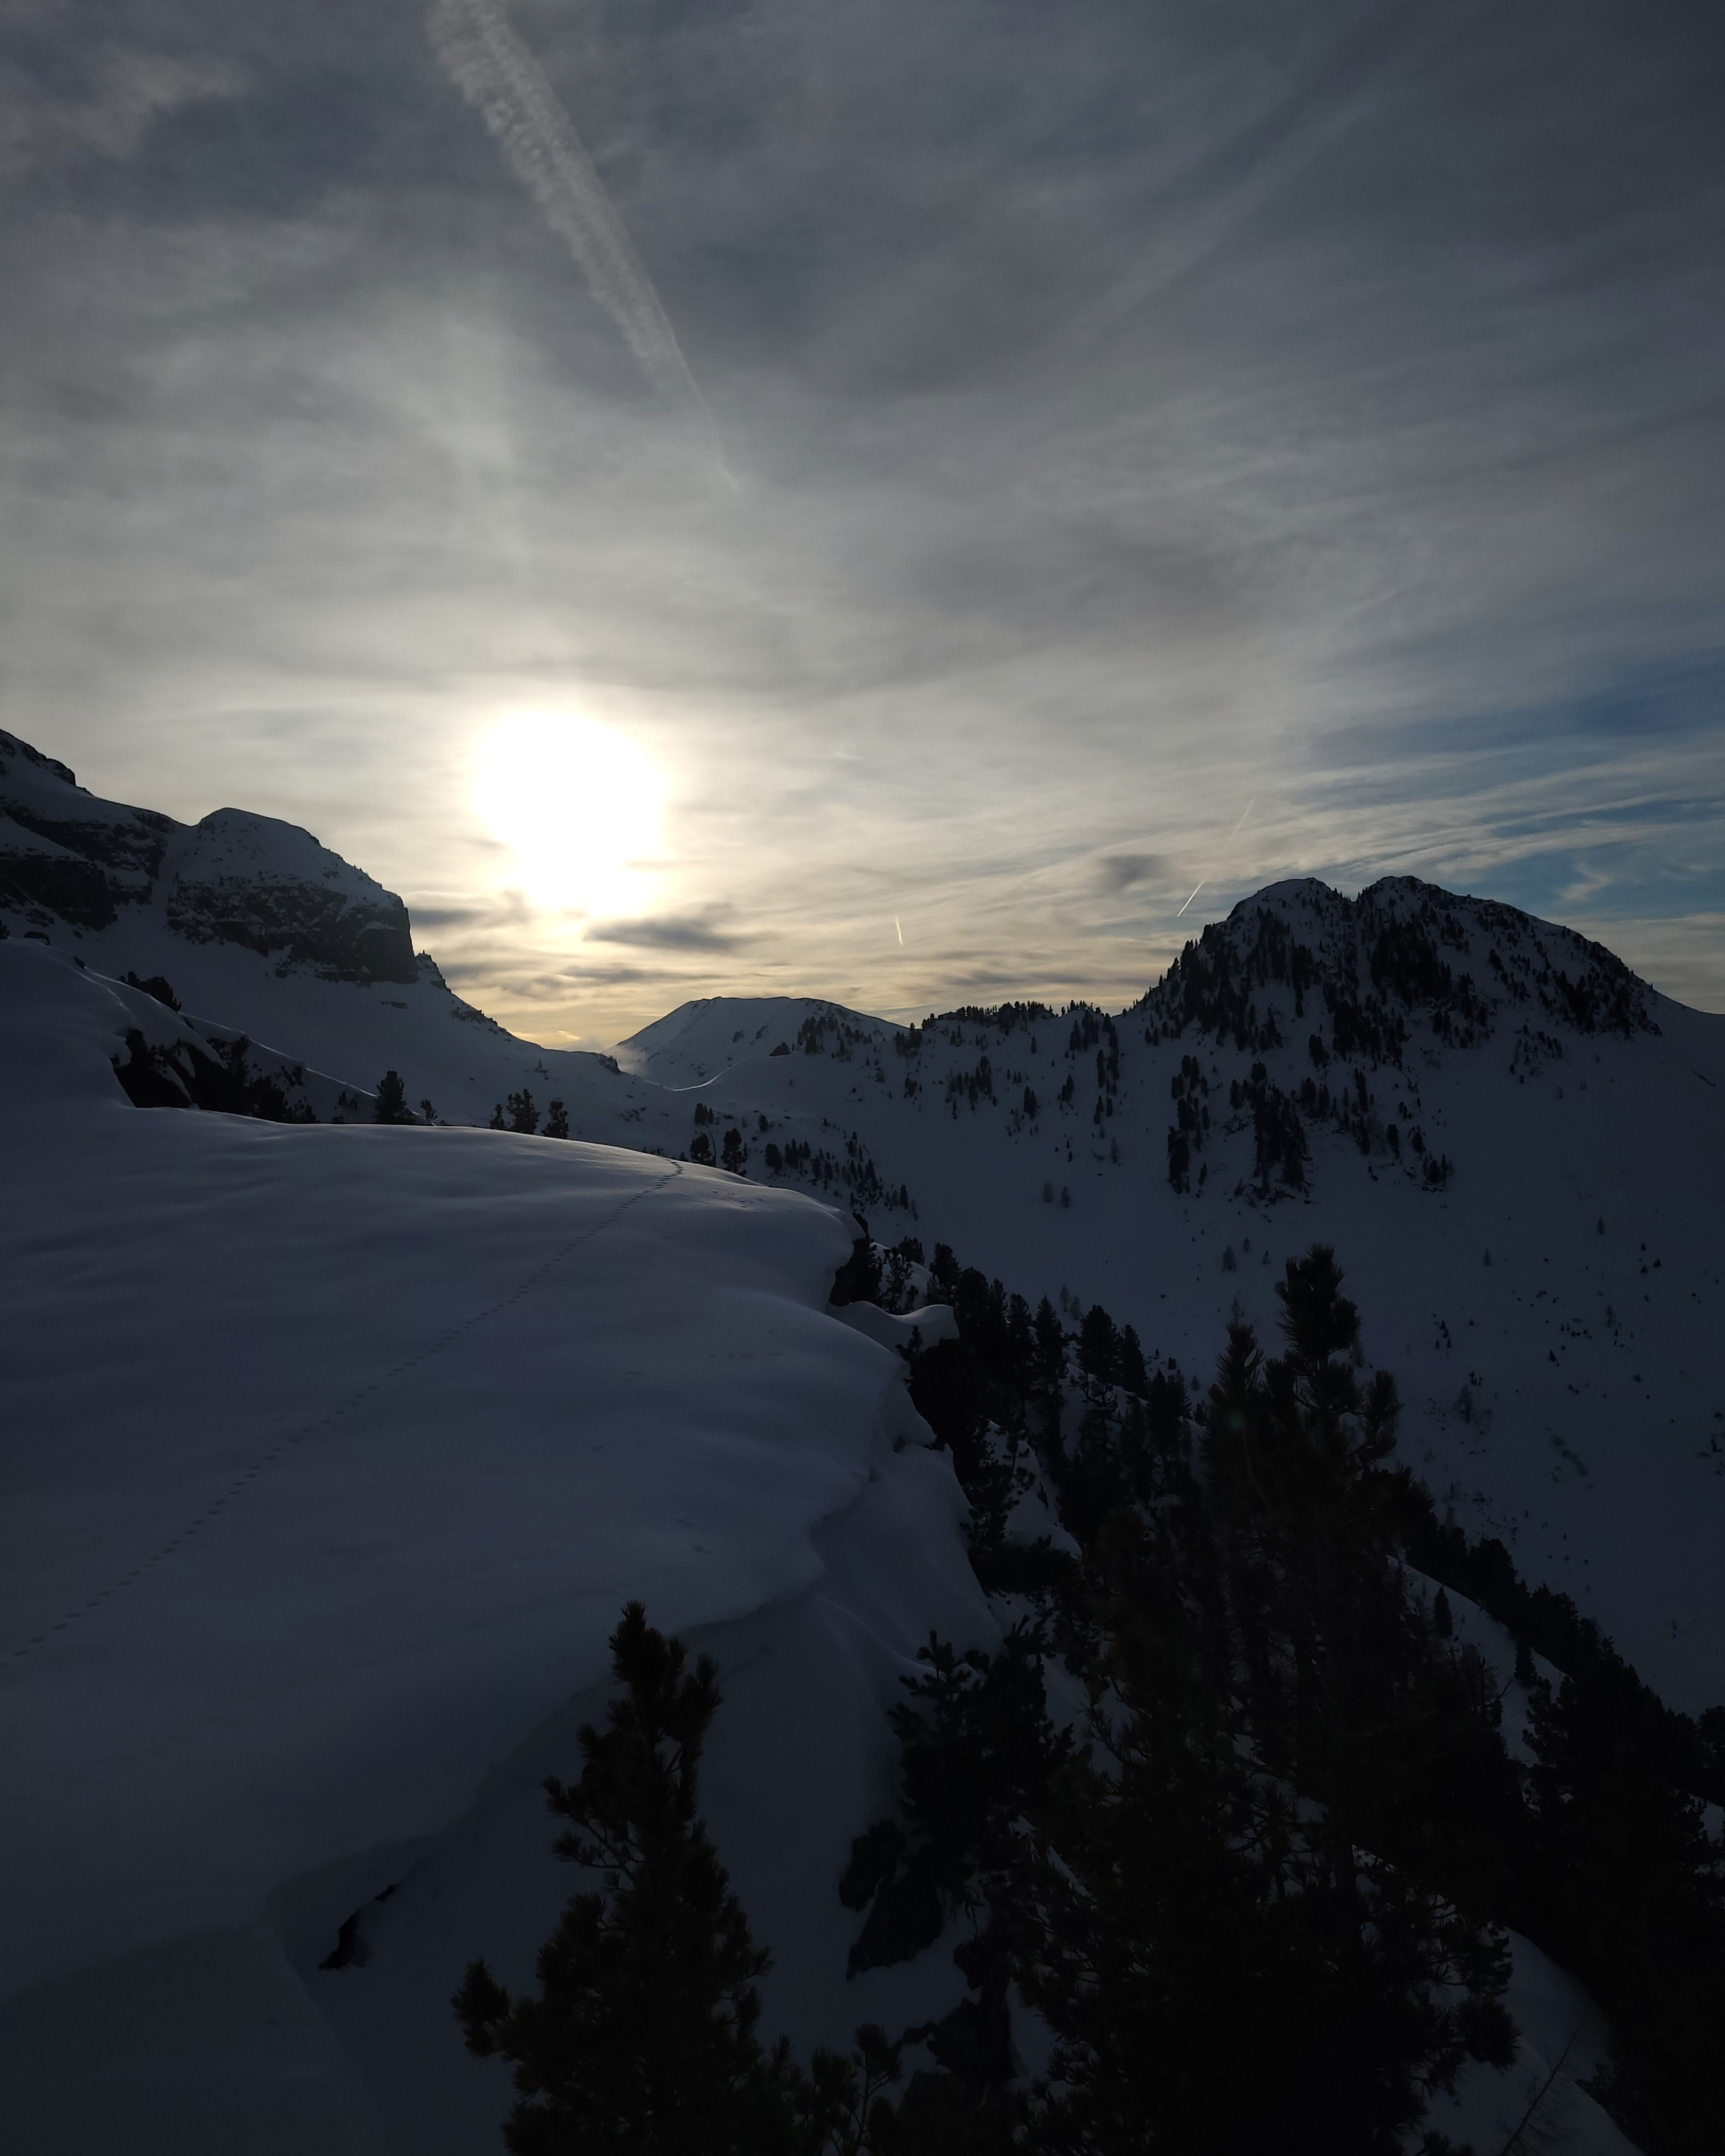
\includegraphics[width=\textwidth]{images/foto_sole.jpg}
        \caption{Vista durante il cammino.}
    \end{subfigure}
    \hfill
    \begin{subfigure}[b]{0.45\textwidth}
        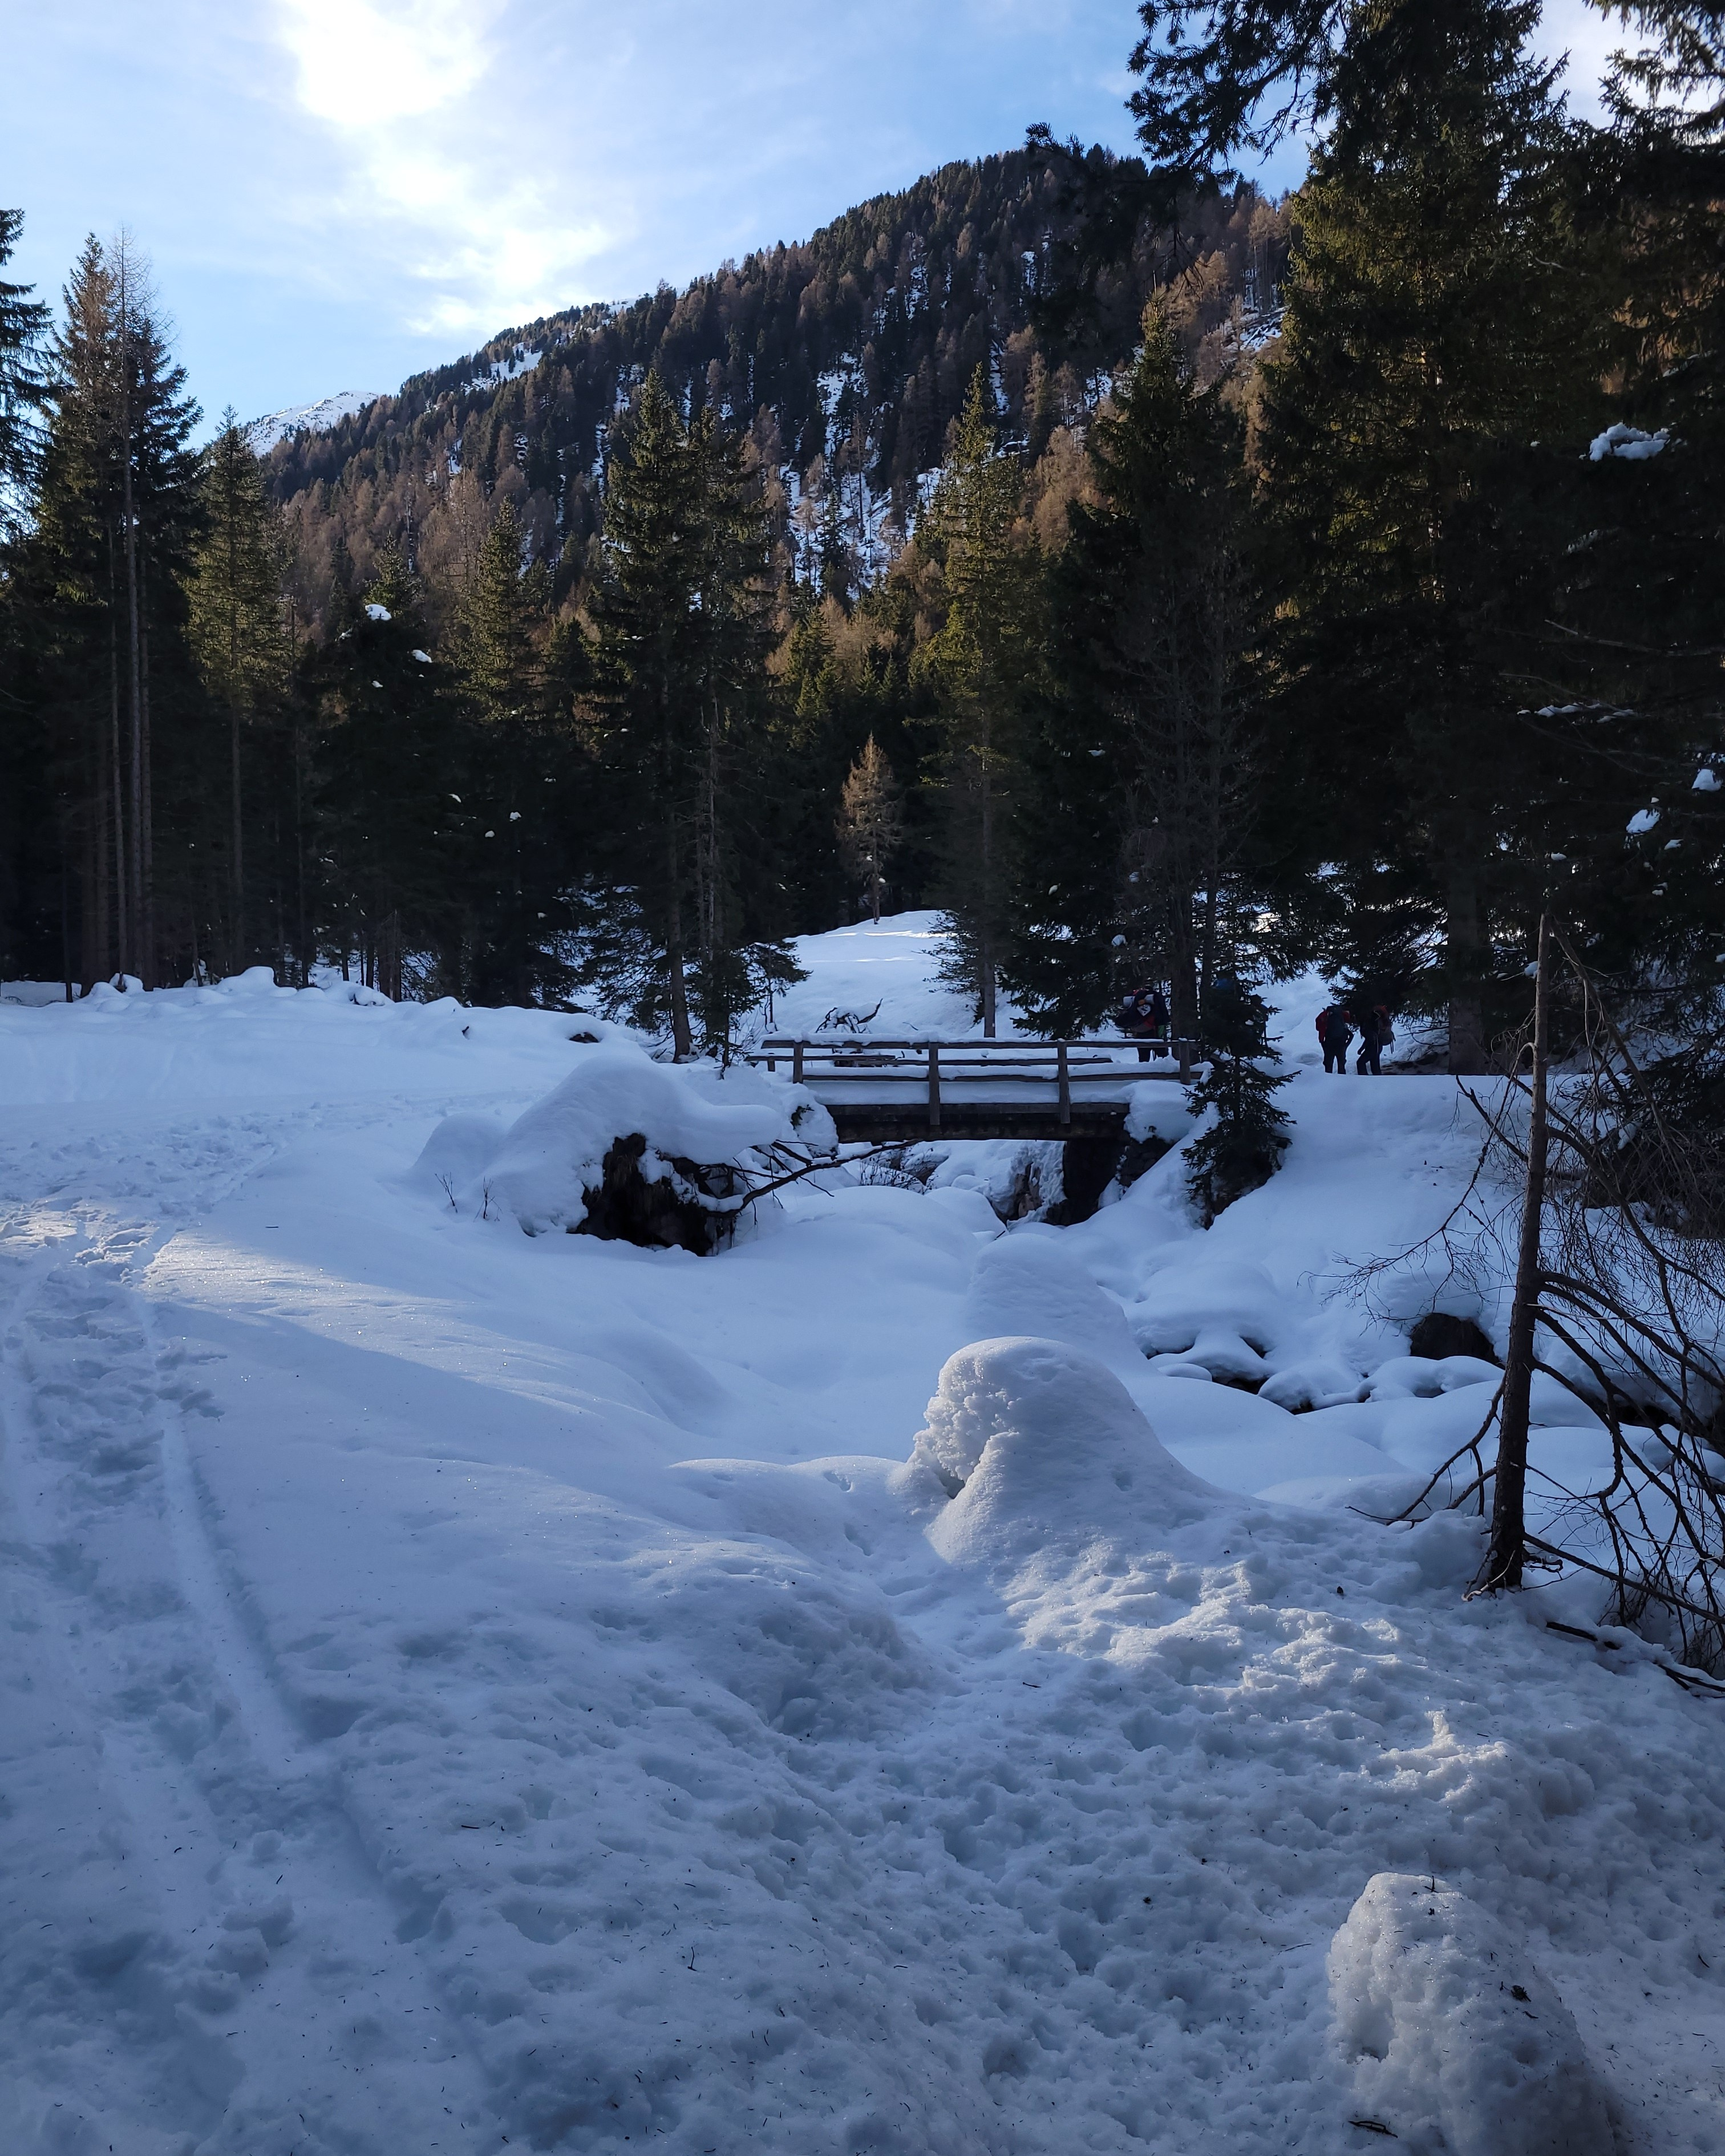
\includegraphics[width=\textwidth]{images/foto_ponte.jpg}
        \caption{Ponte nel sentiero.}
    \end{subfigure}
    \hfill

    % setto il counter delle figure
    \setcounter{figure}{2}
    \caption{Selezione di fotografie del percorso.}
\end{figure}


\clearpage

\section*{Tabella riepilogativa delle caratteristiche}

\begin{tabularx}{\textwidth}{|l|X|}
\hline
\rowcolor{gray!15} \textbf{Caratteristica} & \textbf{Dettaglio} \\
\hline
Regione & Trentino-Alto Adige\\
Comune / Provincia & Trento / Valfloriana \\
Gruppo montuoso & Catena del Lagorai \\
Quota & 1887 m s.l.m. \\
Apertura & Non gestito, sempre aperto \\
Posti letto effettivi & 5 brande \\
Presenze in visita & 15 persone \\
Arredi & Tavolo, panche, stufa \\
Acqua & \ding{51} - Rubinetto esterno con acqua proveniente da fonte\\
Servizi igienici & \ding{51} - Latrina poco sotto\\
Copertura telefonica & \ding{55} - Poca e solo in determinati punti\\
Manutenzione / proprietà & Pubblico / CAI / Comune / Volontari\\
Visitato il & 27-28-29 dicembre 2022\\
\hline
\end{tabularx}

\end{document}
